\documentclass[a5paper, 10pt]{article}

% Текст
\usepackage[utf8]{inputenc} % UTF-8 кодировка
\usepackage[russian]{babel} % Русский язык
\usepackage{indentfirst} % красная строка в первом параграфе в главе
% Отображение страниц
\usepackage{geometry} % размеры листа и отступов
\geometry{
	left=12mm,
	top=25mm,
	right=15mm,
	bottom=17mm,
	marginparsep=0mm,
	marginparwidth=0mm,
	headheight=10mm,
	headsep=7mm,
	nofoot}
\usepackage{afterpage,fancyhdr} % настройка колонтитулов
\pagestyle{fancy}
\fancypagestyle{style}{ % создание нового стиля style
	\fancyhf{} % очистка колонтитулов
	\fancyhead[LO, RE]{Вариант №20} % название документа наверху
	\fancyhead[RO, LE]{\leftmark} % название section наверху
	\fancyfoot[RO, LE]{\thepage} % номер страницы справа внизу на нечетных и слева внизу на четных
	\renewcommand{\headrulewidth}{0.25pt} % толщина линии сверху
	\renewcommand{\footrulewidth}{0pt} % толцина линии снизу
}
\fancypagestyle{plain}{ % создание нового стиля plain -- полностью пустого
	\fancyhf{}
	\renewcommand{\headrulewidth}{0pt}
}
\fancypagestyle{title}{ % создание нового стиля title -- для титульной страницы
	\fancyhf{}
	\fancyhead[C]{{\footnotesize
			Министерство образования и науки Российской Федерации\\
			Федеральное государственное автономное образовательное учреждение высшего образования
	}}
	\fancyfoot[C]{{\large 
			Санкт-Петербург, 2023
	}}
	\renewcommand{\headrulewidth}{0pt}
}

% Математика
\usepackage{amsmath, amsfonts, amssymb, amsthm} % Набор пакетов для математических текстов
%\usepackage{dmvnbase} % мехматовский пакет latex-сокращений
\usepackage{cancel} % зачеркивание для сокращений
% Рисунки и фигуры
\usepackage[pdftex]{graphicx} % вставка рисунков
\usepackage{wrapfig, subcaption} % вставка фигур, обтекая текст
\usepackage{caption} % для настройки подписей
\captionsetup{figurewithin=none,labelsep=period, font={small,it}} % настройка подписей к рисункам
% Рисование
\usepackage{tikz} % рисование
\usepackage{circuitikz}
\usepackage{pgfplots} % графики
% Таблицы
\usepackage{multirow} % объединение строк
\usepackage{multicol} % объединение столбцов
% Остальное
\usepackage[unicode, pdftex]{hyperref} % гиперссылки
\usepackage{enumitem} % нормальное оформление списков
\usepackage{listings} % для добавления кода
\setlist{itemsep=0.15cm,topsep=0.15cm,parsep=1pt} % настройки списков
% Теоремы, леммы, определения...
\theoremstyle{definition}
\newtheorem{Def}{Определение}
\newtheorem*{Axiom}{Аксиома}
\theoremstyle{plain}
\newtheorem{Th}{Теорема}
\newtheorem{Lem}{Лемма}
\newtheorem{Cor}{Следствие}
\newtheorem{Ex}{Пример}
\theoremstyle{remark}
\newtheorem*{Note}{Замечание}
\newtheorem*{Solution}{Решение}
\newtheorem*{Proof}{Доказательство}
% Свои команды
\newcommand{\comb}[1]{\left[\hspace{-4pt}\begin{array}{l}#1\end{array}\right.\hspace{-5pt} } % совокупность уравнений
% Титульный лист
\usepackage{csvsimple-l3}
\newcommand*{\titlePage}{
	\thispagestyle{title}
	\begingroup
	\begin{center}
		%		{\footnotesize
			%			Министерство образования и науки Российской Федерации\\
			%			Федеральное государственное автономное образовательное учреждение высшего образования
			%		}
		%		
		\vspace*{6ex}
		
		{\small
			САНКТ-ПЕТЕРБУРГСКИЙ НАЦИОНАЛЬНЫЙ ИССЛЕДОВАТЕЛЬСКИЙ УНИВЕРСИТЕТ ИТМО
		}
		
		\vspace*{2ex}
		
		{\normalsize
			Факультет систем управления и робототехники
		}
		
		\vspace*{15ex}
		
		{\Large \bfseries 
			Лабораторная работа  №1
		}

                     \vspace*{2ex}
{\Large \bfseries 
			"Интеграл Римана"
		}

                     \vspace*{2ex}
		
		{\normalsize
			по дисциплине "Математический анализ"
		}
                     \vspace*{2ex}
		
		{\normalsize \bfseries
			вариант №20
		}
	\end{center}
	\vspace*{20ex}
	\begin{flushright}
		{\large 
			\underline{Выполнила}: студентка гр. \textbf{R3138}\\
			\begin{flushright}
				\textbf{Нечаева А. А.}\\
			\end{flushright}
		}
		
		\vspace*{5ex}
		
		{\large 
			\underline{Преподаватель}: \textit{Бойцев А. А.}
		}
	\end{flushright}	
	\newpage
	\setcounter{page}{2}
	\endgroup}

\begin{document}
           \newpage
	\titlePage
	\pagestyle{style}
           \section{Аналитическая часть}
           \subsection{Доказательство существование интеграла по Риману}
$f(x) = cos(2x) \in C[0,\, \frac{\pi}{2}]$, следовательно, выполняется достаточное условие интегрируемости функции по Риману - непрерывная на отрезке функция интегрируема на нем. \\	
	\subsection{Вычисление интеграла Римана по определению}
Рассмотрим поведение функции $f(x) = cos(2x)$ на отрезке $[0,\, \frac{\pi}{2}]$ 

 Разобьем интеграл на сумму двух
\begin{equation}
\int\limits_0^\frac{\pi}{2} cos(2x) \,dx = \int\limits_0^\frac{\pi}{4} cos(2x) \,dx + \int\limits_\frac{\pi}{4}^\frac{\pi}{2} cos(2x) \,dx 
\end{equation}
Заметим, что поведение фунции на отрезках  $[0, \frac{\pi}{4}]$ и  $[ \frac{\pi}{4},\frac{\pi}{2} ]$ симметрично с точностью до знака. Поэтому вычислим интеграл
\begin{equation}
\int\limits_0^\frac{\pi}{4} cos(2x) \,dx
\end{equation}
Для этого введем равномерное разбиение $\tau$ отрезка $[0, \frac{\pi}{4}]$
\begin{equation}
0=\frac{\pi 0}{4 n}, \frac{\pi 1}{4 n}, ... , \frac{\pi (n - 1)}{4 n}, \frac{\pi n}{4 n}=\frac{\pi}{4 }
\end{equation}
Длинной отрезка разбиения является величина $\Delta x_i$ 
\begin{equation}
\Delta x_i = x_i - x_{i-1}= \frac{\pi}{4 n}
\end{equation}
В качестве оснащения $\xi$ выберем правые границы отрезков разбиения
\begin{equation}
\xi_i =\frac{\pi i}{4 n}
\end{equation}
Запишем интегральную сумму $\sigma_\tau (f, \xi)$
\begin{equation}
\sigma_\tau (f, \xi)= \sum\limits_{i=1}^n f(\xi_i) \cdot \Delta x_i = \sum\limits_{i=1}^n \left(cos\frac{\pi i}{2n}\right) \cdot \frac{\pi}{4 n}
\end{equation}
Отдельно найдем значение S
\begin{equation}
S = \sum\limits_{i=1}^n \left( cos\frac{\pi i}{2n}\right)
\end{equation}
$2 \cdot cos\frac{\pi}{2n} \cdot S = 2 cos\frac{\pi}{2n} \cdot cos\frac{\pi}{2n} + 2 cos\frac{\pi}{2n} \cdot cos\frac{2 \pi}{2n} + ... + 2 cos\frac{\pi}{2n} \cdot cos\frac{n\pi}{2n} = $ \\
 \\
 $ = 1 + cos\frac{2 \pi}{2n} + cos\frac{\pi}{2n} + cos\frac{3 \pi}{2n} + cos\frac{2 \pi}{2n} + cos\frac{4 \pi}{2n} + ... + cos\frac{(n-1) \pi}{2n} + cos\frac{(n+1) \pi}{2n}= $ \\
 \\
 $ = 1 + 2 \cdot S - cos\frac{\pi}{2n}-cos\frac{\pi}{2}+ cos\frac{(n+1)\pi}{2n} \rightarrow S =\frac{cos\frac{\pi}{2n}+ sin \frac{\pi}{2n} - 1}{2 \left(1 - cos\frac{\pi}{2n}\right)} $\\
\\
Упрощая, получаем
\begin{equation}
 S = \frac{1 - 2\left(sin\frac{\pi}{4n}\right)^2+ sin \frac{\pi}{2n} -1}{4 \left(sin\frac{\pi}{4n}\right)^2} = \frac{cos \frac{\pi}{4n}}{2 sin\frac{\pi}{4n}} - \frac{1}{2} = \frac{1}{2tg\frac{\pi}{4n}} - \frac{1}{2}
\end{equation}
Вычислим значение интеграла Римана по определению
\begin{equation}
\int\limits_0^\frac{\pi}{4} cos(2x) \,dx = \lim\limits_{n \to +\infty}  \sigma_{\tau} (f,  \xi) = \frac{\pi}{8}\lim\limits_{n \to +\infty} \left( \frac{1}{n tg\frac{\pi}{4n}} - \frac{1}{n} \right)= \frac{\pi}{8}\lim\limits_{n \to +\infty} \frac{4n}{n\pi} = \frac{1}{2}
\end{equation}
 \subsection{Вычисление определенного интеграла по формуле Ньютона-Лейбница}
Найдем соответствующий интеграл по формуле Ньютона-Лейбница
\begin{equation}
\int\limits_a^b f(x) \,dx = F(b) - F(a) = \int\limits_0^\frac{\pi}{4} cos(2x) \,dx =\left. \frac{1}{2}sin2x \right|_0^\frac{\pi}{4} =  \frac{1}{2}
\end{equation}
Значения, одно из которых получено по определению интеграла Римана, а второе - путем применения формулы Ньютона-Лейбница, совпадают. \\
\\
Вернемся к исходному интегралу $\int\limits_0^\frac{\pi}{2} cos(2x) \,dx$ . Воспользовавшись симметрией площадей, ограниченных осью $ X$ и графиком функции $f(x) = cos(2x)$  на отрезках $[0, \frac{\pi}{4}]$ и  $[ \frac{\pi}{4},\frac{\pi}{2} ]$ вычислим
\begin{equation}
\int\limits_0^\frac{\pi}{2} cos(2x) \,dx = \int\limits_0^\frac{\pi}{4} cos(2x) \,dx + \int\limits_\frac{\pi}{4}^\frac{\pi}{2} cos(2x) \,dx  = \frac{1}{2} - \frac{1}{2} = 0
\end{equation}
Соотвественно, значение, найденное по формуле Ньютона-Лейбница
\begin{equation}
 \int\limits_0^\frac{\pi}{2} cos(2x) \,dx =\left. \frac{1}{2}sin2x \right|_0^\frac{\pi}{2} = 0
\end{equation}
 \subsection{Вывод формулы теоретической погрешности интеграла и его приближения для правых и левых точек}
Запишем погрешность интеграла в общем виде
\begin{equation}
\left|R_n\right| = \left| \sigma_\tau (f, \xi) - \int\limits_a^b f(x) \,dx \right| =  \left| \sigma_{\tau} (f, \xi) - \sum\limits_{i=1}^n \int\limits_{x_{i-1}}^{x_{i}} f(x) \,dx \right|
\end{equation}
Рассмотрим случай оснащения правыми границами отрезков. Интегральную сумму представим в следующем виде
\begin{equation}
\sigma_\tau (f, \xi) = \sum\limits_{i=1}^n f(x_{i})(x_{i} - x_{i-1}) = \sum\limits_{i=1}^n \int\limits_{x_{i-1}}^{x_{i}} f(x_{i}) \,dx 
\end{equation}
Погрешность запишем 
\begin{equation}
\left|R_n\right| = \left|\sum\limits_{i=1}^n \int\limits_{x_{i-1}}^{x_{i}} f(x) \,dx - \sum\limits_{i=1}^n \int\limits_{x_{i-1}}^{x_{i}} f(x_{i}) \,dx \right| = \left|\sum\limits_{i=1}^n \int\limits_{x_{i-1}}^{x_{i}} \left( f(x) -  f(x_{i}) \right) \,dx\right|
\end{equation}
Разложим $f(x)$ по формуле Тейлора с остатком в форме Лагранжа в точке $x_0 = x_{i} $
\begin{equation}
f(x) = f(x_{i}) + f'(\phi_i)(x - x_{i}), \phi_i \in [x,  x_i ]
\end{equation}
\begin{equation}
\left|R_n\right| =  \left|\sum\limits_{i=1}^n \int\limits_{x_{i-1}}^{x_{i}}  f'(\phi_i)(x - x_{i})  \,dx\right|
\end{equation}
Заметим, что справедливо неравенство
\begin{multline}
\left|R_n\right| = \left|\sum\limits_{i=1}^n \int\limits_{x_{i-1}}^{x_{i}}  f'(\phi_i)(x - x_{i})  \,dx\right| \leqslant  \sum\limits_{i=1}^n \int\limits_{x_{i-1}}^{x_{i}} \left| f'(\phi_i) (x - x_{i})\right|  \,dx = \\ =\sum\limits_{i=1}^n  \left| f'(\phi_i) \left. \frac{(x - x_{i})^2}{2} \right|_{x_{i-1}}^{x_{i}}\right| = \sum\limits_{i=1}^n  \left| f'(\phi_i)  \frac{(x_{i} - x_{i})^2 - (x_{i-1} - x_{i})^2}{2} \right| = \\ = \sum\limits_{i=1}^n  \left| f'(\phi_i) \right| \frac{ (x_{i} - x_{i-1})^2}{2}
\end{multline}
Оценим $\left| f'(\phi_i)\right| \leqslant\max\limits_{x \in [a,\,b]} \left|f'(x)\right| $ и получим выражение
\begin{equation}
\left|R_n\right| \leqslant  \max\limits_{x \in [a,\,b]} \left|f'(x)\right|  \sum\limits_{i=1}^n  \frac {(x_i - x_{i-1})^2}{2} 
\end{equation}
\begin{equation}
\left|R_n\right| \leqslant \max\limits_{x \in [a,\,b]} \left|f'(x)\right|  \sum\limits_{i=1}^n  \frac {(x_i - x_{i-1})^2}{2} = \max\limits_{x \in [a,\,b]} \left|f'(x)\right|   n \frac {(\frac{b - a}{n})^2}{2}
\end{equation}
Выражение выше аналогично данному в методических указаниях для оснащения левыми или правыми точками
\begin{equation}
\left|R_n\right| \leqslant \max\limits_{x \in [a,\,b]} \left|f'(x)\right|  \frac {(b - a)^2}{2n}
\end{equation}
Найдем значение погрешности для $f(x) = cos(2x)$ на отрезке $[0, \frac{\pi}{4}]$
\begin{equation}
\left|R_n\right| \leqslant \max\limits_{x \in [0,\, \frac{\pi}{4}]} \left| -2sin(2x)\right|  \frac {(\frac{\pi}{4})^2}{2n} = \frac {\pi^2}{16n}
\end{equation}
Вернемся к рассмотрению функции по полном отрезке и найдем значение погрешности для $f(x) = cos(2x)$ на отрезке $[0, \frac{\pi}{2}]$
\begin{equation}
\left|R_n\right| \leqslant \max\limits_{x \in [0,\, \frac{\pi}{2}]} \left| -2sin(2x)\right|  \frac {(\frac{\pi}{2})^2}{2n} = \frac {\pi^2}{4n}
\end{equation}
 \subsection{Вывод формулы теоретической погрешности интеграла и его приближения для центральных точек}
Запишем интегральную сумму для случая оснащения центральными точками
\begin{equation}
\sigma_\tau (f, \xi) = \sum\limits_{i=1}^n f \left( \frac{x_{i} + x_{i-1}}{2} \right)(x_{i} - x_{i-1}) = \sum\limits_{i=1}^n \int\limits_{x_{i-1}}^{x_{i}} f \left(\frac{x_{i} + x_{i-1}}{2} \right) \,dx 
\end{equation}
Соотвественно, погрешность
\begin{equation}
\left|R_n\right| = \left|\sum\limits_{i=1}^n \int\limits_{x_{i-1}}^{x_{i}} \left( f(x) -  f \left( \frac{x_{i} + x_{i-1}}{2} \right) \right) \,dx\right|
\end{equation}
Разложим функцию $f(x)$ по формуле Тейлора с остатком в форме Лагранжа $x_0 = \frac{x_{i} + x_{i-1}}{2}$
\begin{multline}
f(x) = f \left( \frac{x_{i} + x_{i-1}}{2} \right) + f' \left( \frac{x_{i} + x_{i-1}}{2} \right) \left(x - \frac{x_{i} + x_{i-1}}{2} \right) +\\ + \frac{f'' \left(\phi_i \right)}{2} \left(x - \frac{x_{i} + x_{i-1}}{2} \right)^2
\end{multline}
Вернемся к погрешности
\begin{equation}
\left|R_n\right| =\left| \sum\limits_{i=1}^n \int\limits_{x_{i-1}}^{x_{i}} \left( f' \left( \frac{x_{i} + x_{i-1}}{2} \right) \left(x - \frac{x_{i} + x_{i-1}}{2} \right) + \frac{f'' \left(\phi_i \right)}{2} \left(x - \frac{x_{i} + x_{i-1}}{2} \right)^2 \right) \,dx \right| 
\end{equation}
Вычислим значение интеграла, разбив его на сумму двух и посчитав их по отдельности
\begin{multline}
 f' \left( \frac{x_{i} + x_{i-1}}{2} \right) \int\limits_{x_{i-1}}^{x_{i}}  \left(x - \frac{x_{i} + x_{i-1}}{2} \right) \,dx  = \left.  f' \left( \frac{x_{i} + x_{i-1}}{2} \right) \frac{\left(x - \frac{x_{i} + x_{i-1}}{2}\right)^2}{2}  \right|_{x_{i-1}}^{x_{i}} = \\ =  f' \left( \frac{x_{i} + x_{i-1}}{2} \right) \frac{\left(x_{i} - \frac{x_{i} + x_{i-1}}{2}\right)^2 - \left(x_{i-1} - \frac{x_{i} + x_{i-1}}{2}\right)^2}{2} = \\ = f' \left( \frac{x_{i} + x_{i-1}}{2} \right) \frac{\left(\frac{x_{i} - x_{i-1}}{2}\right)^2 - \left( \frac{x_{i-1} - x_{i}}{2}\right)^2}{2} = 0
\end{multline}
\\
\begin{multline}
\frac{f'' \left(\phi_i \right)}{2} \int\limits_{x_{i-1}}^{x_{i}} \left(x - \frac{x_{i} + x_{i-1}}{2} \right)^2  \,dx = \frac{f'' \left(\phi_i \right)}{2} \left. \frac{\left(x - \frac{x_{i} + x_{i-1}}{2} \right)^3}{3} \right|_{x_{i-1}}^{x_{i}} = \\ = \frac{f'' \left(\phi_i \right)}{6} \left( \left(\frac{x_{i} - x_{i-1}}{2}\right)^3 - \left( \frac{x_{i-1} - x_{i}}{2}\right)^3 \right) = \frac{f'' \left(\phi_i \right)}{3}  \left(\frac{x_{i} - x_{i-1}}{2}\right)^3
\end{multline}
В результате получаем
\begin{equation}
\left|R_n\right| = \sum\limits_{i=1}^n \frac{\left| f'' \left(\phi_i \right) \right| }{3} \left(\frac{x_{i} - x_{i-1}}{2} \right)^3  
\end{equation}
Заметим, что $ \left| f'' \left(\phi_i \right) \right| \leqslant \max\limits_{x \in [a,\,b]} \left|f''(x)\right| $  и $x_{i} - x_{i-1} = \frac{b - a}{n}$\\
Перейдем к оценке погрешности
\begin{equation}
\left|R_n\right| \leqslant  \frac{\max\limits_{x \in [a,\,b]} \left|f''(x)\right|}{3} n  \left(\frac{b - a}{2n} \right)^3   = \max\limits_{x \in [a,\,b]} \left|f''(x)\right| \frac{\left(b - a\right)^3}{24 n^2} 
\end{equation}
Найдем значение погрешности  для $f(x) = cos(2x)$ на отрезке $[0, \frac{\pi}{4}]$
\begin{equation}
\left|R_n\right| \leqslant \max\limits_{x \in [0, \frac{\pi}{4}]} \left|-4 cos(2x)\right| \frac{\left(\frac{\pi}{4}\right)^3}{24 n^2} =\frac{\pi^3}{384 n^2}
\end{equation}
Вернемся к исходному отрезку и найдем значение погрешности  для $f(x) = cos(2x)$ на отрезке $[0, \frac{\pi}{2}]$
\begin{equation}
\left|R_n\right| \leqslant \max\limits_{x \in [0, \frac{\pi}{2}]} \left|-4 cos(2x)\right| \frac{\left(\frac{\pi}{2}\right)^3}{24 n^2} =\frac{\pi^3}{48 n^2}
\end{equation}
\newpage
 \section{Практическая часть}
Программа написана на языке Python (Python 3.9) с использованием библиотек Manim (Manim Community v0.17.3), Numpy, и Scipy. Репозиторий на GitHub по \href{https://github.com/a-nechaeva/MathLab}{ссылке}.
\subsection{Запуск программы}
Пример запуска программы через CMD Windows и выбора левых точек оснащения
\begin{lstlisting}
C:\...\mathAn>manim -pql .\cos_integral.py Left
\end{lstlisting}
Для правых точек
\begin{lstlisting}
C:\...\mathAn>manim -pql .\cos_integral.py Right
\end{lstlisting}
И центральных
\begin{lstlisting}
C:\...\mathAn>manim -pql .\cos_integral.py Center
\end{lstlisting}
\subsection{Результаты работы программы}
В результате получены интегральные суммы для оснащения центральными, правыми и левыми точками при различном количестве точек разбиения. Для удобства интегральные суммы подсчитываются на отрезке  $[0, \frac{\pi}{4}]$. Заметим, что значения погрешности $Real \left|R_n \right|$ не привышают значения теоретической $Theory \left|R_n \right|$, что подтверждает правдоподобность полученной оценки.

\begin{figure}[h]
		\begin{center}
                      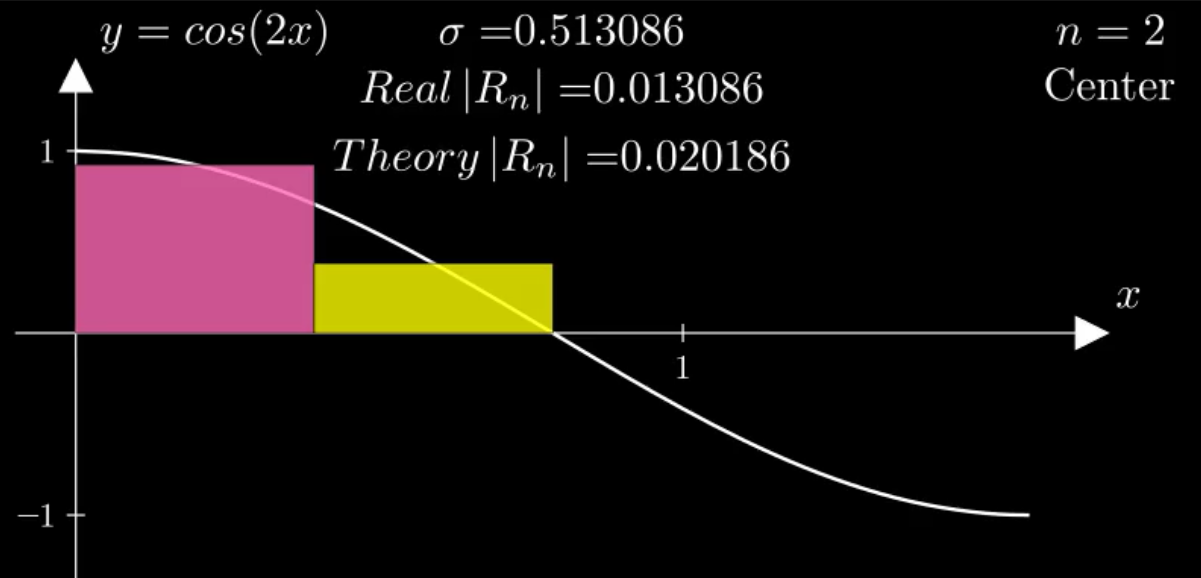
\includegraphics[width=\linewidth]{"./c2.png"}
	           \caption{Для центральных точек при $n=2$}
		\end{center}
	\end{figure}
\begin{figure}
		\begin{center}
                      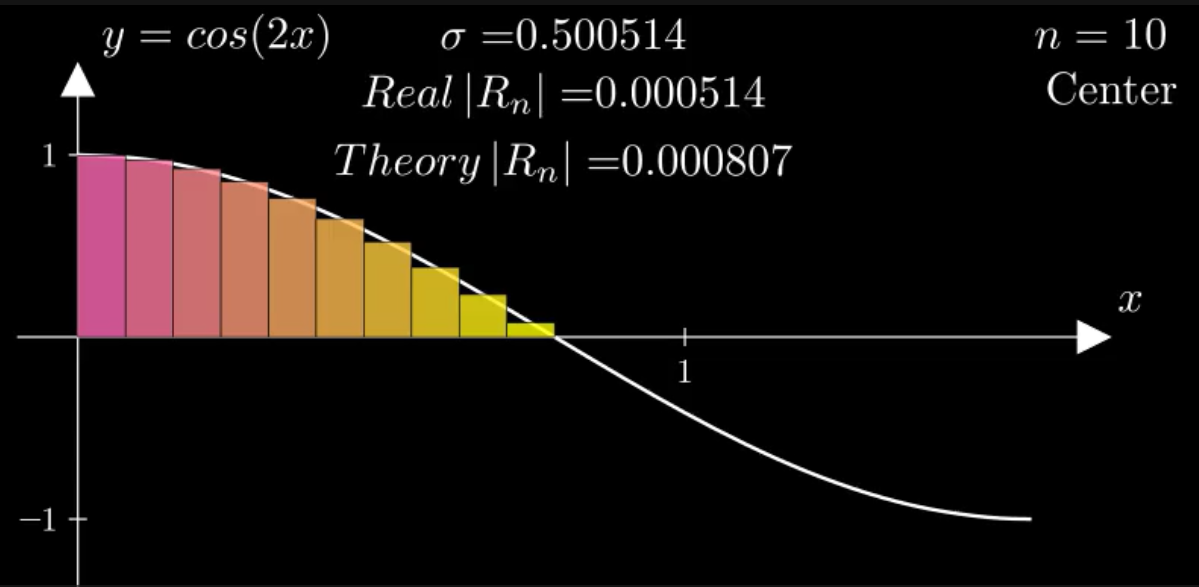
\includegraphics[width=\linewidth]{"./c10.png"}
	           \caption{Для центральных точек при $n=10$}
		\end{center}
	\end{figure}
\begin{figure}
		\begin{center}
                      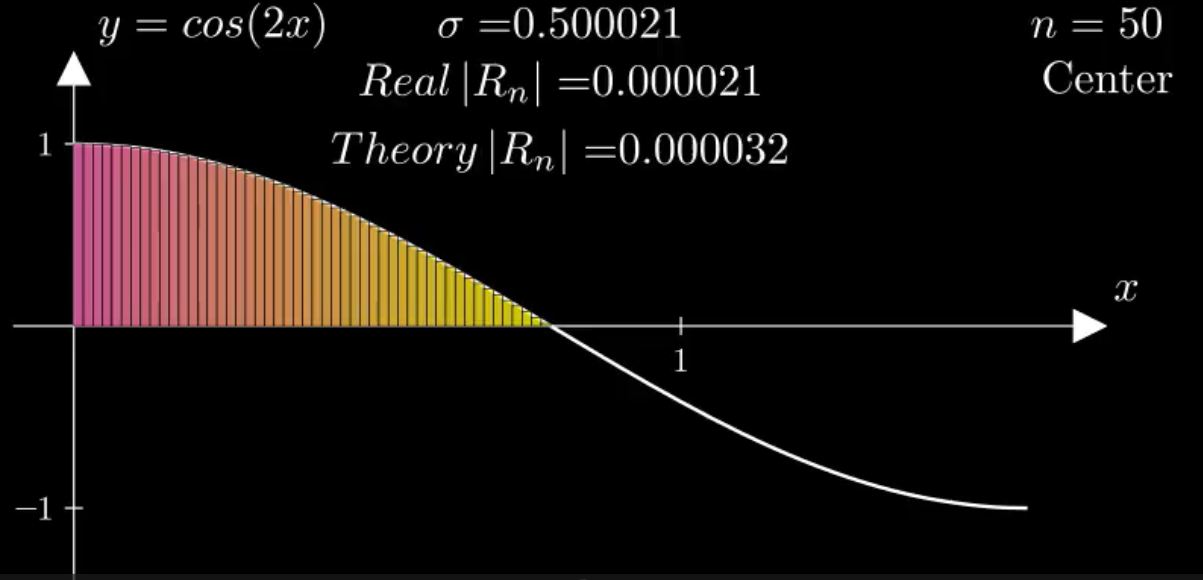
\includegraphics[width=\linewidth]{"./с50.png"}
	           \caption{Для центральных точек при $n=50$}
		\end{center}
	\end{figure}
\begin{figure}
		\begin{center}
                      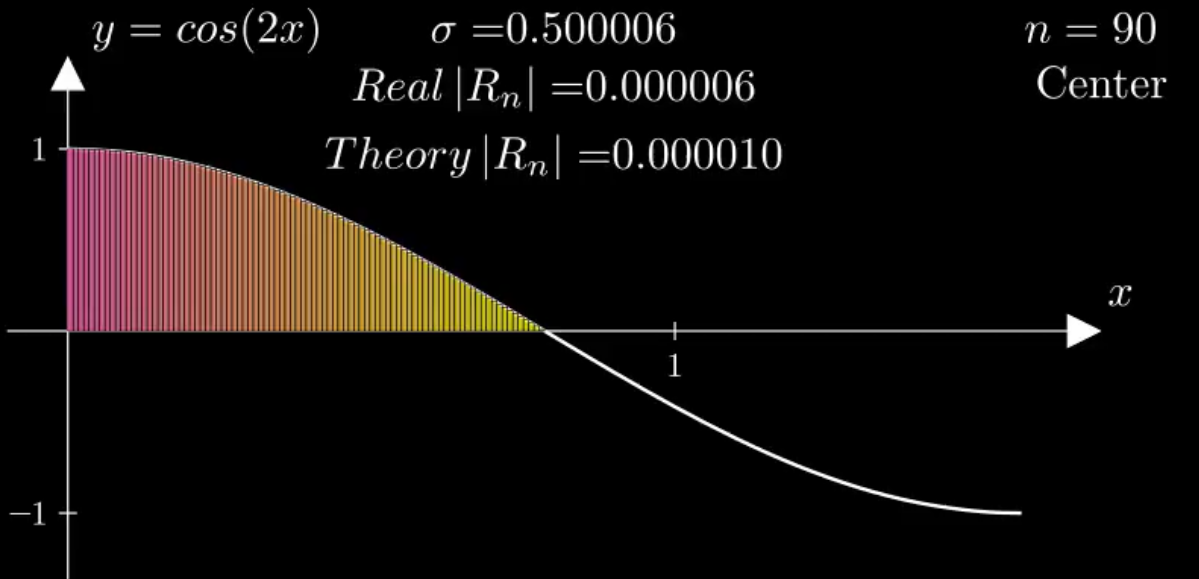
\includegraphics[width=\linewidth]{"./с90.png"}
	           \caption{Для центральных точек при $n=90$}
		\end{center}
	\end{figure}
\begin{figure}
		\begin{center}
                      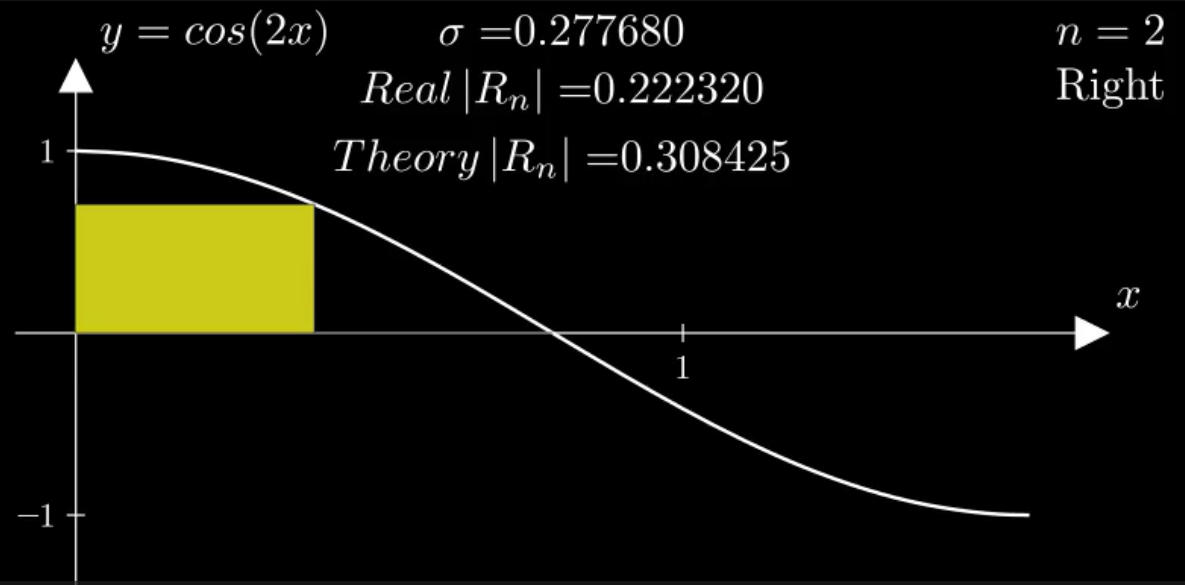
\includegraphics[width=\linewidth]{"./r2.png"}
	           \caption{Для правых точек при $n=2$}
		\end{center}
	\end{figure}
\begin{figure}
		\begin{center}
                      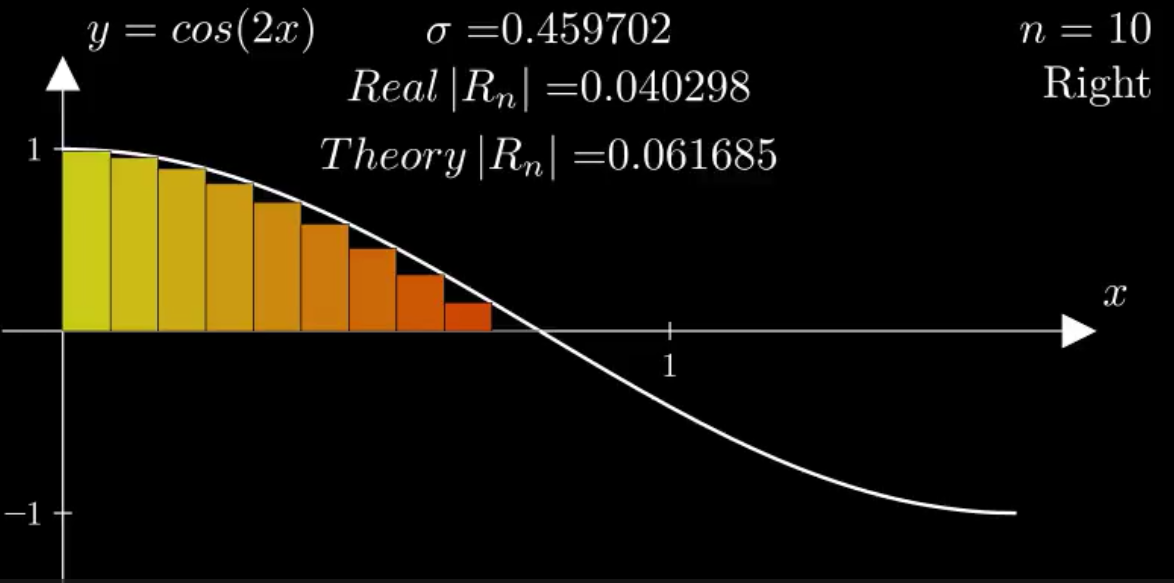
\includegraphics[width=\linewidth]{"./r10.png"}
	           \caption{Для правых точек при $n=10$}
		\end{center}
	\end{figure}
\begin{figure}
		\begin{center}
                      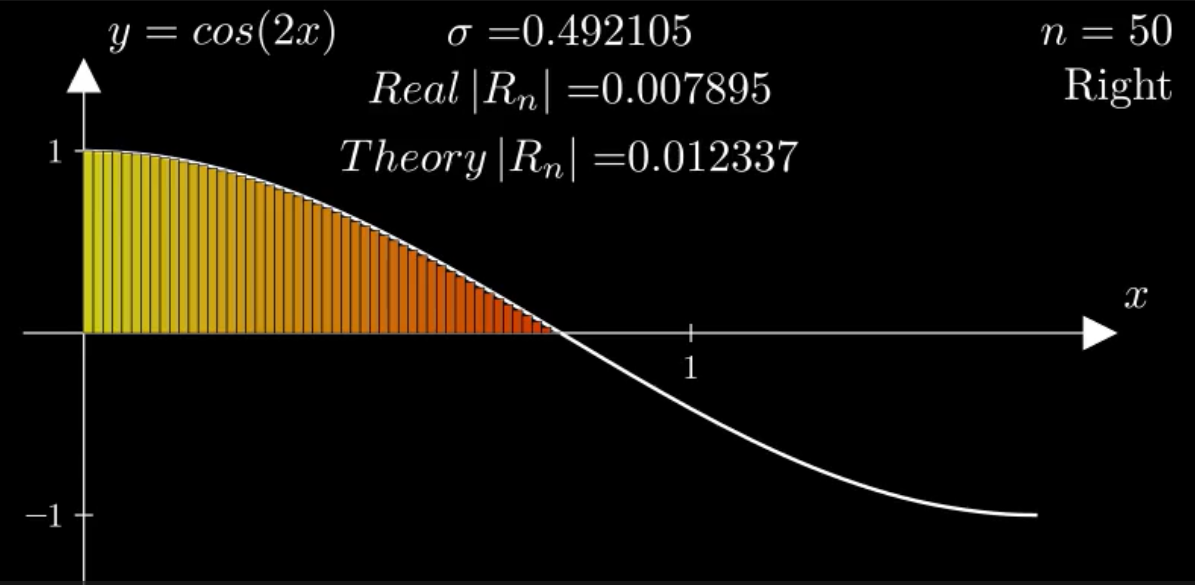
\includegraphics[width=\linewidth]{"./r50.png"}
	           \caption{Для правых точек при $n=50$}
		\end{center}
	\end{figure}
\begin{figure}
		\begin{center}
                      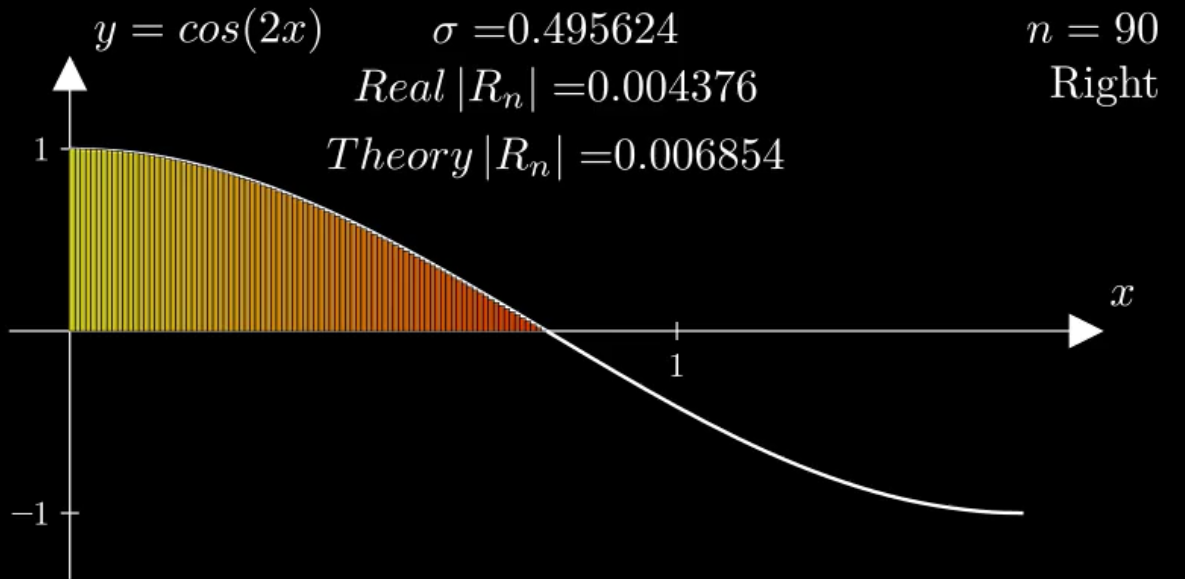
\includegraphics[width=\linewidth]{"./r90.png"}
	           \caption{Для правых точек при $n=90$}
		\end{center}
	\end{figure}
\begin{figure}
		\begin{center}
                      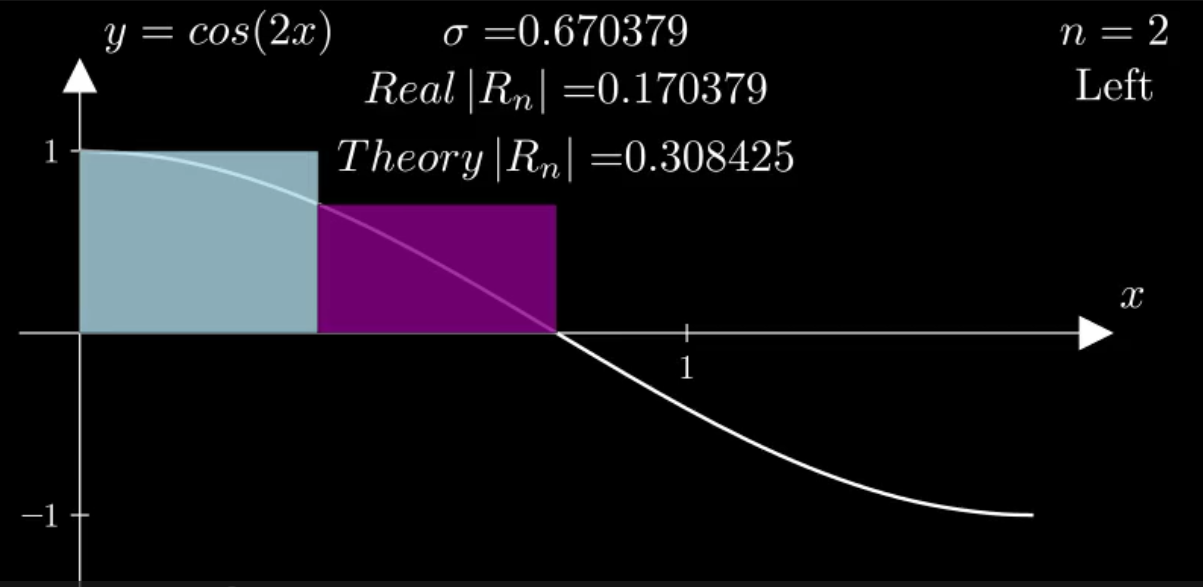
\includegraphics[width=\linewidth]{"./l2.png"}
	           \caption{Для левых точек при $n=2$}
		\end{center}
	\end{figure}
\begin{figure}
		\begin{center}
                      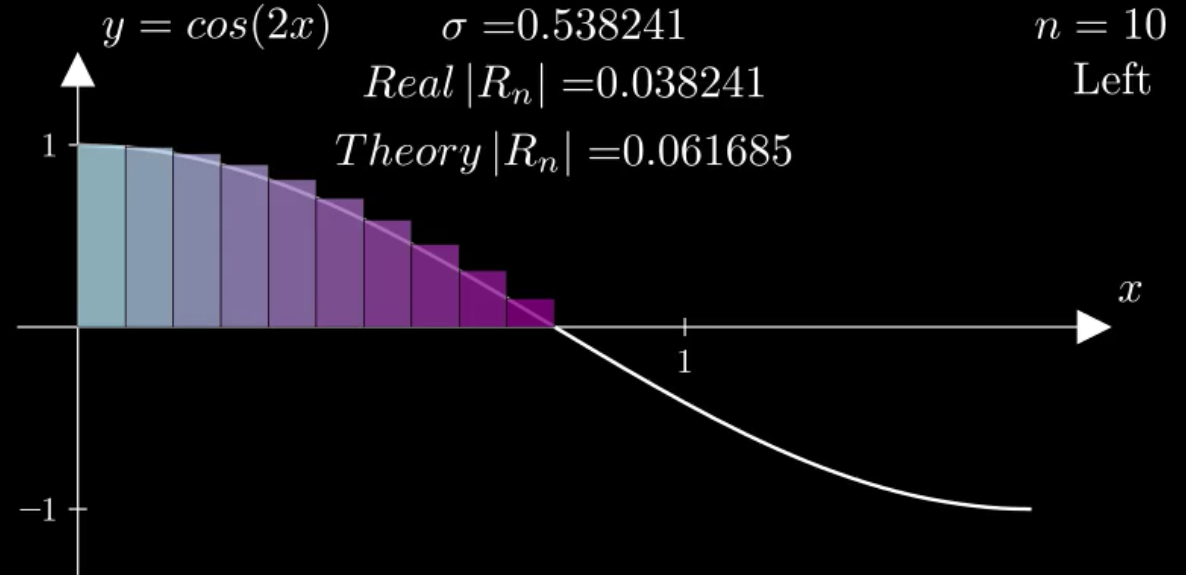
\includegraphics[width=\linewidth]{"./l10.png"}
	           \caption{Для левых точек при $n=10$}
		\end{center}
	\end{figure}
\begin{figure}
		\begin{center}
                      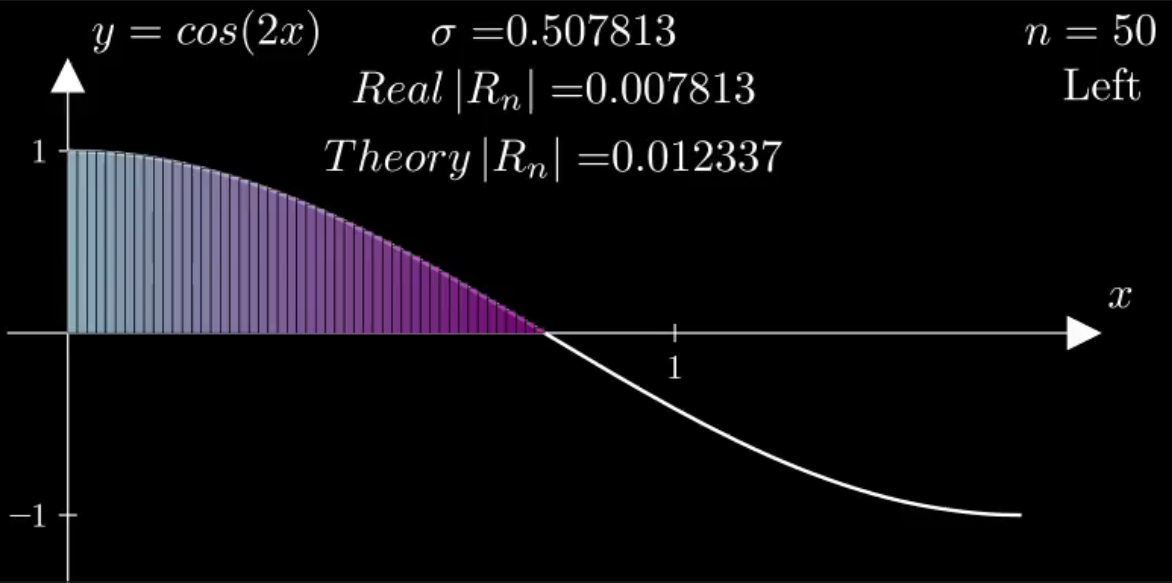
\includegraphics[width=\linewidth]{"./l50.png"}
	           \caption{Для левых точек при $n=50$}
		\end{center}
	\end{figure}
\begin{figure}
		\begin{center}
                      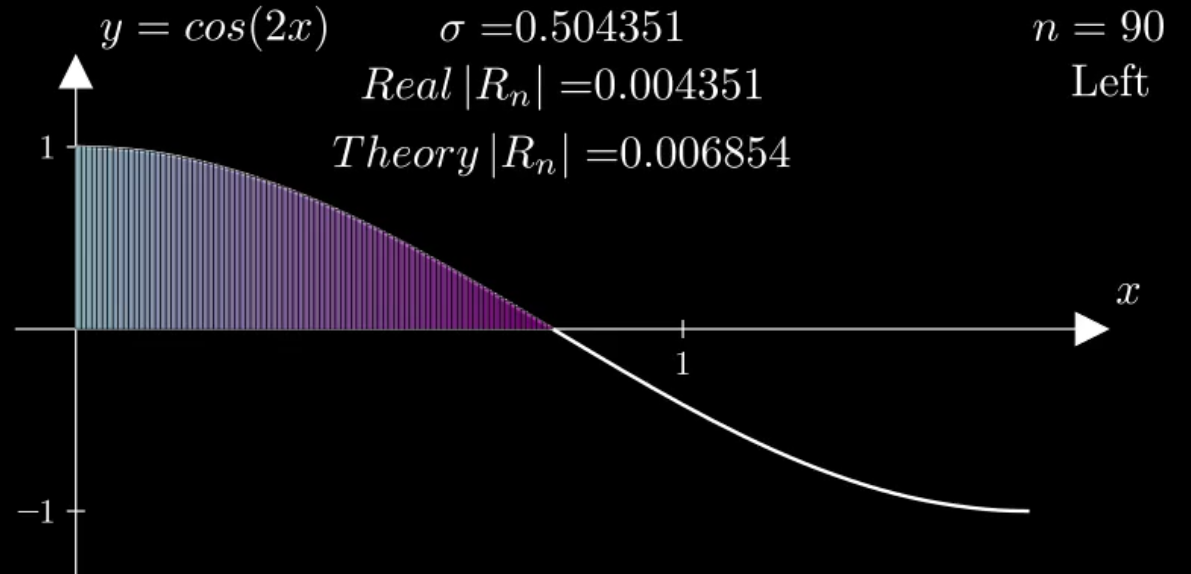
\includegraphics[width=\linewidth]{"./l90.png"}
	           \caption{Для левых точек при $n=90$}
		\end{center}
	\end{figure}
\end{document}











